\chapter[Lecture 24]{}\label{lec24}

\section*{Fermi surface}
\begin{quote}
Extended zone scheme $\to$ Different bands in different zone.

Reduced zone scheme $\to$ All bands in first zone.

Periodic zone scheme $\to$ every band in every zone.
\end{quote}
\begin{figure}[H]
\centering
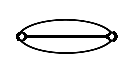
\includegraphics{images/lecture24/fig9.eps}

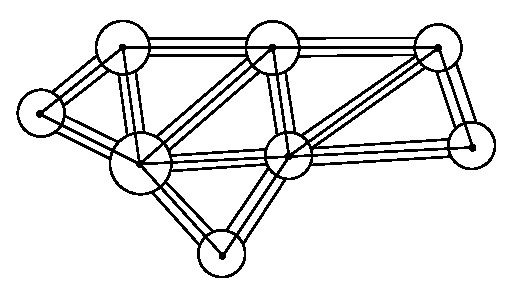
\includegraphics{images/lecture24/fig10.eps}
\end{figure}

\newpage

\begin{itemize}
\itemsep=0pt
\item[(i)] Interaction of electrons with periodic potential creates energy gap at zone boundary.

\item[(ii)] Fermi surface intersects zoen boundary perpendicularly.

\item[(iii)] Crystal potentials round out sharp corners in FS.

\item[(iv)] Total volume enclosed by FS depends only on electron concentration and is independent of lattice interactions.
\end{itemize}

Draw spheres at every reciprocal lattice point $\to$ volume represent electron concentration.
\begin{itemize}
\itemsep=0pt
\item[(a)] If a $k$-print lies at least in one sphere $\to$ first zone

\item[(b)] $k$-point at least in two spheres $\to$ second zone.

\item[(c)] $k$-point at least in three spheres $\to$ third zone.
\end{itemize}
\begin{figure}[H]
\centering
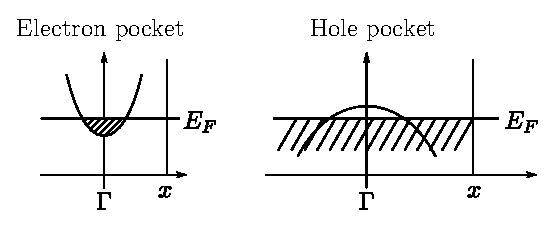
\includegraphics{images/lecture24/fig11.eps}
\end{figure}

Enclosed area contains unoccupied $k$-points.

Experimental Determination of Fermi surface.
\begin{tabbing}
\phantom{N}Direct method \=$\to$ Phto emission (ARPES)\\[4pt]
Indirect method \>$\to$ de Haas - Van Alphen effect\\[4pt]
                \>$\to$ Shubnikow-de Haas effect\\[4pt]
                \>$\to$ Anomalous skin effect\\[4pt]
                \>$\to$ magneto resistance\\[4pt]
                \>$\to$ magneto-acoustic effect
\end{tabbing}

In a magnetic field, momentum of a particle with charge $q$ is
$$
P=P_{\text{kin}}+P_{\text{field}}=\hbar k+\dfrac{qA}{C}\quad \overrightarrow{B}=\overrightarrow{V}\times \overrightarrow{A}
$$

Following Onsagar and Lifshitz approach, we assume that orbits in a magnetic field is quantized by Bohr-Sommerfeld relation
$$
\oint p-d\overrightarrow{r}=(n+\gamma)2\pi \hbar
$$
$n\to$ integer, $\nu\to$ phase correction $=\dfrac{1}{2}$ for electrons.
$$
\oint p\cdot dr=\oint \hbar k\cdot dr+\dfrac{q}{c}\oint A\cdot dr
$$
Now $\hbar k=p=\dfrac{q}{c}\overrightarrow{r}\times \overrightarrow{B}$
$$
\therefore\quad \oint \hbar k\cdot dr=\dfrac{q}{c}\oint r\times B\cdot dr=-\dfrac{qB}{C}\cdot \oint r\times dr=-\dfrac{2q}{C}\phi
$$
$\phi\to$ magnetic flux within the orbit in real space
$$
\oint r\times dr = 2\times \text{ (area enclosed by the orbit)}
$$

\section*{Stokes Theorem}

Now,
\begin{align*}
\frac{q}{c}\oint A\cdot A\cdot dr &= \dfrac{q}{c}\int \nabla\times A\cdot dS \text{ (area integral)}\\
&= \frac{q}{c}\int B\cdot ds=\dfrac{q}{c}\phi\\
\therefore \ \oint p\cdot dr &= -\dfrac{q}{c}\phi = (n+\gamma)2\pi\hbar
\end{align*}
$$
\therefore\quad \fbox{$\phi_{n}=(n+\gamma)\dfrac{2\pi\hbar c}{e}$}\quad q=-e\text{ for electrons.}
$$
$2\pi\hbar c/e\simeq 4.14\times 10^{-7}$ Gauss $m^{2}$ or $Tm^{2}$

Now, we know  $p=\dfrac{q}{c}r\times B\Rightarrow \hbar\overrightarrow{k}=\dfrac{q}{c}\overrightarrow{r}\times \overrightarrow{B}$
$$
\Rightarrow \text{ taking magnitude, } \fbox{$\Delta r=\dfrac{\hbar c}{eB}\cdot \Delta k$}
$$
$\therefore$ Area $A_{n}$ in real space is related are {\em $S_{n}$ in reciprocal space}
\begin{gather*}
a, A_{n}=\left(\dfrac{\hbar C}{eB}\right)^{2}S_{n}\\
\therefore\quad \phi_{n}=\left(\dfrac{\hbar C}{e}\right)^{2}-\dfrac{1}{B}\cdot S_{n}=(n+\gamma)2\pi \hbar C/e\\
\therefore\quad \fbox{$S_{n}=(n+\gamma)\dfrac{2\pi e}{\hbar C}B$}
\end{gather*}
$\to$ Area of an orbit in $k_{n}$, $k_{y}$ space.
\begin{align*}
\therefore\quad \Delta &=\text{ area between successive orbits.}\\
&= S_{n}-S_{n-1}=\dfrac{2\pi eB}{\hbar C}
\end{align*}
If the specimen is a square of side $L$.

This area occupied by a single orbital $=\left(\dfrac{2\pi}{L}\right)^{2}$.

$\therefore$ Degeneracy of a single level $=\dfrac{2neB}{\hbar C}\cdot \left(\dfrac{L}{2\pi}\right)^{2}=\rho B=D_{n}$
$$
\rho=\dfrac{eL^{2}}{2\pi\hbar C}
$$
Magnetic levels are called Landan levels.
\begin{figure}[H]
\centering
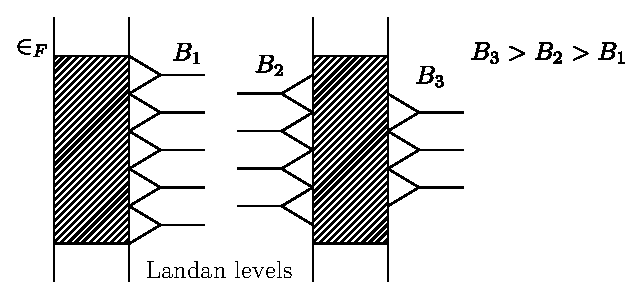
\includegraphics{images/lecture24/fig12.eps}
\end{figure}

Increase $B$ gradually

Degeneracy increases.

Separation of the levels increases
\begin{gather*}
E_{n}=\left(n-\frac{1}{2}\right)\hbar w_{C}\quad n=1,2,3,\ldots\\
\fbox{$w_{C}=\dfrac{eB}{m^{v}e}$}
\end{gather*}

\begin{tabbing}
Completely filled level \=$\to$ Partially filled\\[3pt]
\>$\to$ Completely filled ... etc.
\end{tabbing}

Critical field at which all the levels are filled
$$
n\rho B_{n}=N\quad N=\text{ total no. of electrons.}
$$
{\bf Energy:} Total Energy for fully filled levels.
$$
=\sum\limits^{n}_{i=1}D_{i}\hbar w_{C}(i-Y_{2})=\frac{1}{2}D_{n}\hbar w_{C}n^{2}
$$

Energy of the partially filled level
$$
=\hbar w_{C}\left(n+\frac{1}{2}\right)(N-nD)
$$
\begin{align*}
\therefore\quad \text{Total energy} &= \frac{1}{2}D\hbar w_{C}n^{2}+\hbar w_{C}\left(n+\frac{1}{2}\right)(N-nD)\\[3pt]
&= \hbar w_{C}\left[\frac{1}{2}Dn^{2}+\left(n+\frac{1}{2}\right)N-n\left(n+\frac{1}{2}\right)D\right]\\[3pt]
&= \hbar w_{C}\left[\left(n+\frac{1}{2}\right)N-\frac{1}{2}D(n+1)\right]
\end{align*}
\begin{align*}
D &= \dfrac{eL^{2}}{2\pi \hbar C}\cdot B\\[3pt]
w_{C} &= \dfrac{eB}{m^{*}C}
\end{align*}
\begin{figure}[H]
\centering
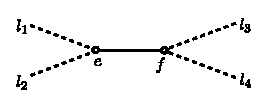
\includegraphics{images/lecture24/fig13.eps}
\end{figure}

